\taughtsession{Lecture}{Sets}{2024-01-23}{17:00}{Janka}{}

\section{Introduction}
\textit{Sets} underpin maths and Computer Science. A set is a collection of objects, which are called the elements (also known as members of the set). For example, a set of the numbers 1, 3, 8; or the collection of students in a class born in March. There are two characteristics of sets:
\begin{enumerate}
    \item There are no repeated occurrences of elements
    \item There is no particular order of the elements
\end{enumerate}

\section{Set Notation}
The elements of a set are enclosed in braces with their names being denoted by a \textit{letter}, for example:
\[A = \{1, 2, 3\}, \quad C=\{Portsmouth, Brighton, London\}\]

There are two ways that we can describe the members of a set. We can \textit{list the elements} which is mainly used for finite sets, for example:
\[A = \{3, 6, 9, 12\}\]

Alternatively, we can \textit{specify a property} that all the elements in the set have in common. The `$|$' character is read `such that', sometimes `$:$' is used in it's place. For example:
\[B = \{x | x \mathrm{\ is\ a\ multiple\ of\ 3\ and\ } 0 < x < 15\}\]
We can also use \textit{three dots} to informally denote a sequence of elements that we don't wish to write down, for example:
\[C = \{1, \ldots, 10\}\]

\subsection{Sets of Numbers}
There are some reserved letters to denote specific sets of numbers in maths. These are shown below:
\begin{itemize}
    \item $\mathbb{N}$ (or $N$) is used for the set of natural numbers (integers $>=$ 0). $\mathbb{N} = \{0, 1, 2, 3, 4, \ldots \}$
    \item $\mathbb{Z}$ (or $Z$) is used for the set of integers. $\mathbb{N} = \{\ldots, -1, 0, 1, \ldots \}$
    \item $\mathbb{Q}$ (or $Q$) is used for the set of rational numbers (number which can be expressed as a quotient or fraction). $\displaystyle \mathbb{Q} = \{0, \frac{1}{2}, \frac{1}{3}, \frac{1}{4}, \ldots \}$
    \item $\mathbb{R}$ (or $R$) is used for the set of real numbers. $\mathbb{R} = \{\displaystyle \ldots, -1, 0, \frac{1}{2}, \ldots \}$
\end{itemize}

\subsection{Elements of a Set}
We can use the $\in$ symbol to denote if an element is a member of a given set. For example, if $x$ is a member of $S$ - then we can say:
\[x \in S\]
The symbol $\notin$ denotes an element is not a member of a given set. For example, if $y$ is \textbf{not} a member of $S$ - then we can say:
\[y \notin S\]

\subsection{Many Ways to Say The Same Thing}
There are several ways of describing the same set, for example for the set $S$ of \textit{odd integers}:
\begin{align*}
    S &= \{\ldots, -5, -3, -1, 1, 3, 5, \ldots\}\\
    &= \{x | x \mathrm{\ is\ an\ odd\ integer\ } \}\\
    &= \{x | x=2k+1 \mathrm{\ for\ some\ integer\ } k \}\\
    &= \{x | x = 2k+ 1 \mathrm{\ for\ some\ } k \in \mathbb{Z}\}\\
    &= \{2k+1|k \in \mathbb{Z}\}
\end{align*}

The phrase ``for some [integers $K$]'', means ``for all [integers $k$]''

\subsection{Empty Sets}
Where a set has \textit{no elements}, it is called an empty set or null set. It's denoted with the $\emptyset$ symbol, for example:
\[\emptyset = \{ \}\]

\subsection{Finite \& Infinite Sets}
If the number of elements in the set is fixed (for example when counting the elements at a fixed rate for a set amount of time), then the set is \textit{finite}. If the set $X$ is finite, then we call $|X|$ the \textit{cardinality} of $X$ therefore:
\[|X| = \mathrm{number\ of\ elements\ in\ }X \]
If the counting never stops then $X$ is an infinite set.

\subsection{Subsets}
A subset is where one set's elements are entirely present in another set. There are three conditions we need to know about:
\begin{itemize}
    \item $A \subseteq B$: $A$ is a subset of $B$ therefore every element in $A$ is also in $B$.
    \item $A \nsubseteq B$: $A$ is not a subset of $B$.
    \item $A \subset B$: $A$ is a proper subset of $B$, therefore $B$ has at least one additional element which is not in $A$.
\end{itemize}

\subsection{Equality of Sets}
Two sets are \textit{equal} if they have exactly the same elements. This is denoted by writing $A = B$. Where $A = B$, the following conditions are also true:
\begin{itemize}
    \item $A \subseteq B$ for every $a$ if $a \in A$, then $a \in B$
    \item $B \subseteq A$ for every $b$ if $b \in B$, then $b \in A$
\end{itemize}

\section{Operations on Sets}
Sets can have \textit{operations} performed on them - this will change something about them.
\subsection{Intersection}
The intersection of two sets $A$ and $B$ is defined as:
\[A \cap B = \{ x | x \in A \mathrm{\ and\ } x \in B \}\]
This is the set of elements which appear in both sets only. If we take a Venn Diagram with a set on either side -  its the overlapped elements which would be returned from an intersection operation. For example if $A = \{a, b, c\}$ and $B = \{c, d\}$ then $A \cap B = \{c\}$. 

\begin{figure}[H]
    \centering

    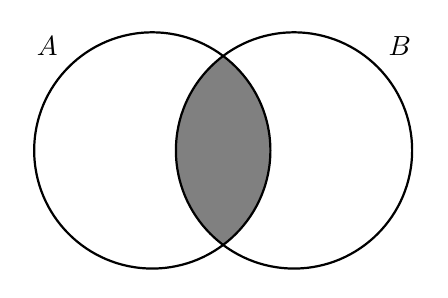
\begin{tikzpicture}[thick,
        set/.style = {circle,
            minimum size = 3cm,
            }]
    
    % Set A
    \node[set,label={135:$A$}] (A) at (0,0) {};
    
    % Set B
    \node[set,label={45:$B$}] (B) at (1.8,0) {};
    
    % Intersection
    \begin{scope}
        \clip (0,0) circle(1.5cm);
        \clip (1.8,0) circle(1.5cm);
        \fill[gray](0,0) circle(1.5cm);
    \end{scope}
    
    % Circles outline
    \draw (0,0) circle(1.5cm);
    \draw (1.8,0) circle(1.5cm);
    
    \end{tikzpicture}  
    \caption{$A \cap B$}  
\end{figure}

\subsection{Disjoint}
If an intersection returns no elements, then the two sets are \textit{disjoint}. This is shown by:
\[A \cap B = \emptyset\]

\subsection{Union}
The \textit{union} of the two sets $A$ and $B$ is defined as:
\[A \cup B = \{ x | x \in A \mathrm{\ or \ } x \in B \}\]
This is the set of elements which are in either $A$ or $B$, this means elements which appear in both are returned. For example, if $A = \{a, b, c\}$ and $B=\{c, d\}$ then $A \cup B = \{a, b, c, d\}$.

\begin{figure}[H]
    \centering

    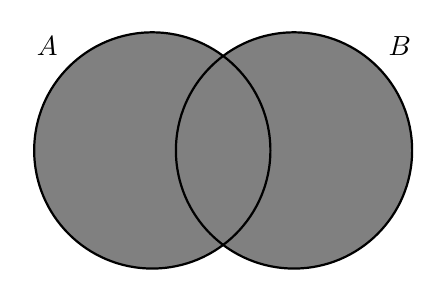
\begin{tikzpicture}[thick,
        set/.style = {circle,
            minimum size = 3cm,
            fill=gray
            }]
    
    % Set A
    \node[set,label={135:$A$}] (A) at (0,0) {};
    
    % Set B
    \node[set,label={45:$B$}] (B) at (1.8,0) {};
    
    % Intersection
    \begin{scope}
        \clip (0,0) circle(1.5cm);
        \clip (1.8,0) circle(1.5cm);
        \fill[gray](0,0) circle(1.5cm);
    \end{scope}
    
    % Circles outline
    \draw (0,0) circle(1.5cm);
    \draw (1.8,0) circle(1.5cm);
    
    \end{tikzpicture}  
    \caption{$A \cup B$}  
\end{figure}

\subsection{Difference}
The \textit{difference} between two sets, $A$ and $B$ is defined as:
\[A \setminus B = \{ x | x \in A \mathrm{\ or \ } x \in B\}\]
This is the set of elements which are in $A$ but not in $B$, so could be represented as $A-B$. Note that $A \setminus B \neq B \setminus A$.

\begin{minipage}{0.45\textwidth}
    \begin{figure}[H]
        \centering
    
        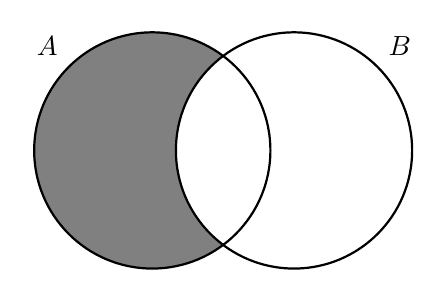
\begin{tikzpicture}[thick,
            set/.style = {circle,
                minimum size = 3cm,
                }]
        
        % Set A
        \node[set,fill=gray,label={135:$A$}] (A) at (0,0) {};
        
        % Set B
        \node[set,label={45:$B$}] (B) at (1.8,0) {};
        
        % Intersection
        \begin{scope}
            \clip (0,0) circle(1.5cm);
            \clip (1.8,0) circle(1.5cm);
            \fill[white](0,0) circle(1.5cm);
        \end{scope}
        
        % Circles outline
        \draw (0,0) circle(1.5cm);
        \draw (1.8,0) circle(1.5cm);
        
        \end{tikzpicture}  
        \caption{$A \setminus B$}  
    \end{figure}
\end{minipage}\hfill
\begin{minipage}{0.45\textwidth}
    \begin{figure}[H]
        \centering
    
        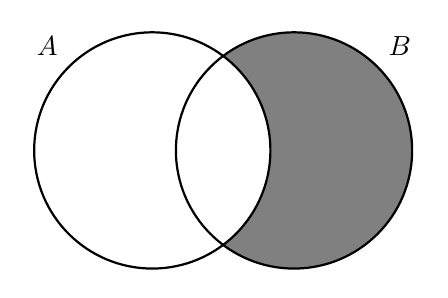
\begin{tikzpicture}[thick,
            set/.style = {circle,
                minimum size = 3cm,
                }]
        
        % Set A
        \node[set,label={135:$A$}] (A) at (0,0) {};
        
        % Set B
        \node[set,fill=gray,label={45:$B$}] (B) at (1.8,0) {};
        
        % Intersection
        \begin{scope}
            \clip (0,0) circle(1.5cm);
            \clip (1.8,0) circle(1.5cm);
            \fill[white](0,0) circle(1.5cm);
        \end{scope}
        
        % Circles outline
        \draw (0,0) circle(1.5cm);
        \draw (1.8,0) circle(1.5cm);
        
        \end{tikzpicture}  
        \caption{$B \setminus A$}  
    \end{figure}
\end{minipage}

\subsection{Counting Elements In a Set}
If we take $A$ and $B$ to be finite sets, we can calculate the number of elements in the union of $A$ and $B$. The correct way to count this is as follows:
\[|A \cup B| = |A| + |B| - |A\cap B|\]
We have to minus $|A \cap B|$ from the sum because otherwise it is as though we are counting it twice due to the fact that we are summing the total number of elements in $A$ and $B$.

\section{Complement}
If we consider that all subsets are the subset of a particular set, $U$ for example (the universe of discourse), then the difference $U\setminus A$ is called the \textit{complement} of $A$ is shown as either $\overline{A}$ or $A'$. For example:
\[A' = \{X | x \in U \mathrm{\ and\ } x \notin A\}\]

\section{Basic Set Properties}
Sets have a number of basic properties - many of these are the same as that for Boolean Expressions
\begin{itemize}
    \item $A \cup \emptyset = A$
    \item $A \cap \emptyset = \emptyset$
    \item $A \cup A = A$
    \item $A \cap A = A$
    \item Commutative
    \begin{itemize}
        \item $A \cup B = B \cup A$
        \item $A \cap B = B \cap A$
    \end{itemize}
    \item Associative
    \begin{itemize}
        \item $(A\cup B)\cup C = A \cup (B\cup C)$
        \item $(A\cap B)\cap C = A \cap (B\cap C)$
    \end{itemize}
    \item Distributive
    \begin{itemize}
        \item $A \cap (B \cap C) = (A \cap B) \cup (A \cap C)$
        \item $A \cup (B \cup C) = (A \cup B) \cap (A \cup C)$
    \end{itemize}
    \item de Morgan's
    \begin{itemize}
        \item $(A \cap B)' = A'\cup B'$
        \item $(A \cup B)' = A'\cap B'$
    \end{itemize}
\end{itemize}

\section{Power Set}
A \textit{power set} is the collection of all subsets of a set, $S$ which is denoted by $P(S)$. For example, if $S = \{a, b, c\}$ then:
\[P(S) = \{ \emptyset, \{a\}, \{b\}, \{c\}, \{a, b\}, \{b, c\}, \{a, c\}, \{a, b, c\} \}\]

\section{Partition}
A \textit{partition} of the set $S$ is a collection of non-empty subsets of set $S$ where every element form $S$ belongs to exactly one member of $S$. This means that the sets are mutually disjoint and that the union of all the sets in the collection results in the original set, $S$. For example, if $S = \{a, b, c, d, e, f\}$ then $\{\{a,e\}, \{c\}, \{f,d\},\{b\}\}$ is a partition of $S$.